\chapter{Evaluation}
\label{cha:evaluation}

The outcome of this thesis will be evaluated according to predetermined functional and non-functional requirements. As already described in the previous sections, this thesis aims to enhance \emph{Privacy}, \emph{Fairness} and \emph{Regulation} in blockchain-based data trading platforms by combining Compute-to-Data and Verifiable Off-chain Computation. These 3 requirements are hard to measure numerically, but the evaluation will include an in-depth discussion about the pros and cons of the proposed system design accordingly, and compared to related work. %However, if I manage to implement verifiable Differential Privacy, privacy gets indeed measurable. % Possibly in form of Threat Model?

The second part of the evaluation will include multiple benchmarks with regards to the practicality, also referred as efficiency, of the proposed system design. Interestingly, \emph{Efficiency} is one of the key features of any digital data trading platform as depicted in chapter \ref{chapter:problem}. %Hence, the result of this evaluation will provide a decent proposition about the real 
Therefore, I will analyze efficiency of on-chain and off-chain components individually, according to costs, scalability and computation time.

One of the most suitable measurements for on-chain components are the costs for each transaction, with regards to gas fees. This is important because the proposed system design is only feasible as a real-world system when costs are reasonably low for the buyer and seller. Since the Blockchain is primarily used to secure the protocol, costs can be compared to conventional buyer and seller protection systems from Ebay or PayPal for example. The most important on-chain transaction will probably be the verification of the zero-knowledge proof, which has to be cheaper than the on-chain execution in the first place. Benchmarks will vary in the size of the dataset and the computation algorithm.

The second analysis includes the evaluation of off-chain components. According to that, the ZKP, which is composed of different phases, is the most important evaluation. I will benchmark especially the time for the one-time setup as well as the proof generation time. The proof generation time will probably have the most impact on the practicality of the proposed system design. Benchmarks will again vary in the size of the dataset and the computation algorithm. Furthermore, I will take the underlying hardware with regards to the computational power into account for this analysis. 

The entire system can be measured in the overall time and amount of exchanged messages until the trade between buyer and seller is completely fulfilled. All benchmarks can be compared to conventional data marketplaces as well as related work, and used to construct suggestions to improve the system design in future work.

THREAT MODEL?
    sybill
    
    
GAS COSTS

EXECUTION TIME

INFRASTRUCTURE COSTS

ZKP'S

REQUIREMENTS

% https://ethgasstation.info/ for price evaluations
\section{Dataset}

\newcommand\inch{\mbox{''}} 

\section{Experimental Setup}

DATASET und USE CASE hier rein?

A simulation of the marketplace is conducted on a single machine, specifically a Macbook Pro (14", 2021) with an Apple Silicon M1 Pro \acrfull{soc}. The \acrshort{soc} consists of an 8-core CPU with 2.06 - 3.22 GHz, 16GB of LPDDR5-6400 unified memory and a pair of 1TB SSD NAND chips with around 5590MB/s write and 4927MB/s read speed.

\section{Computational Costs}

To evaluate the computational performance of system components in the marketplace, on-chain and off-chain computations are observed. Off-chain computations are measured in terms of computation time, the average memory consumption, the number of constraints in the R1CS, and the size of resulting artifacts on the disc. On-chain computations are measured in Gas, to indicate the amount of computational effort, required to execute transactions on the Ethereum blockchain. Therefore, Gas converts into real costs and is denoted in gwei which is a denomination of Ethereum's native coin. Accordingly, 1 gwei is equal to 0.000000001 ETH (10\textsuperscript{-9} ETH). Experiments are conducted with varying numbers of batches as depicted in table \ref{tab:batches}, each comprising 32 records of positive integer values. (Info about SUM + gas units genauer (gas nicht gleich gwei))

\begin{xltabular}{\textwidth}{lccccc}
\toprule
\textbf{Batches [\#]} & \textbf{1} & \textbf{2} & \textbf{4} & \textbf{8} & \textbf{16} \\ \midrule
\endfirsthead

\multicolumn{4}{c}%
{\tablename\ \thetable{} -- continued from previous page}\vspace{2mm} \\
\endhead
    Compile Time [seconds] & 18.575 & 29.035 & 49.465 & 112.135 & 358.286 \\
    Compile Memory [GB] & 2.584 & 3.561 & 4.415 & 3.576 & 2.929 \\
    Constraints [\#] & 278954 & 451900 & 797792 & 1489576 & 2873144 \\
    R1CS Size [GB] & 1.1 & 1.6 & 2.5 & 4.5 & 8.3 \\ \midrule
    Setup Time [seconds] & 18.573 & 25.755 & 44.828 & 84.404 & 178.548 \\
    Setup Memory [GB] & 0.693 & 1.248 & 1.208 & 2.434 & 2.324 \\
    Proving Key Size [MB] & 117 & 169 & 306 & 580 & 1100 \\
    Verification Key Size [KB] & 8 & 16 & 24 & 44 & 64 \\ \midrule
    Witness Time [seconds] & 6.541 & 9.407 & 15.028 & 26.636 & 50.060 \\
    Witness Memory [GB] & 0.034 & 0.043 & 0.058 & 0.089 & 0.148 \\ \midrule
    Proof Time [seconds] & 14.259 & 18.158 & 30.908 & 59.524 & 131.485 \\
    Proof Memory [GB] & 1.240 & 1.730 & 2.694 & 3.439 & 3.029
    \\ \bottomrule
\caption{TODO TODO TODO!} \label{tab:batches}
\end{xltabular}%

The \emph{setup phase} consists of two off-chain computations, i.e. the compilation of the ZoKrates program into a \acrshort{r1cs} and the generation of an evidence key pair, denoted as the \emph{setup} in Figure \ref{fig:setup-phase}. While the number of constraints and the size of the compiled \acrshort{r1cs} behave rather linear, the compilation time increases rather exponentially. Unexpectedly, the pattern of memory consumption during compilation is different for the highest number of batches, which actually consumes the second least amount of memory on average across all numbers of batches. Peaks are reached with 4 and 8 batches at a memory consumption of more than 8 GB. On the test system at most 24 batches are successfully compiled, while the next larger number of batches ran out of memory.

The time for the creation of an evidence key pair (setup), and the size of the proving key are mostly linear to the increasing number of batches. In contrast, the size of the generated verification key increases logarithmically, which is expected to keep the smart contract size and deployment costs low.

\begin{figure}[h]
    \centering
    \begin{subfigure}[t]{0.49\textwidth}
        \centering
        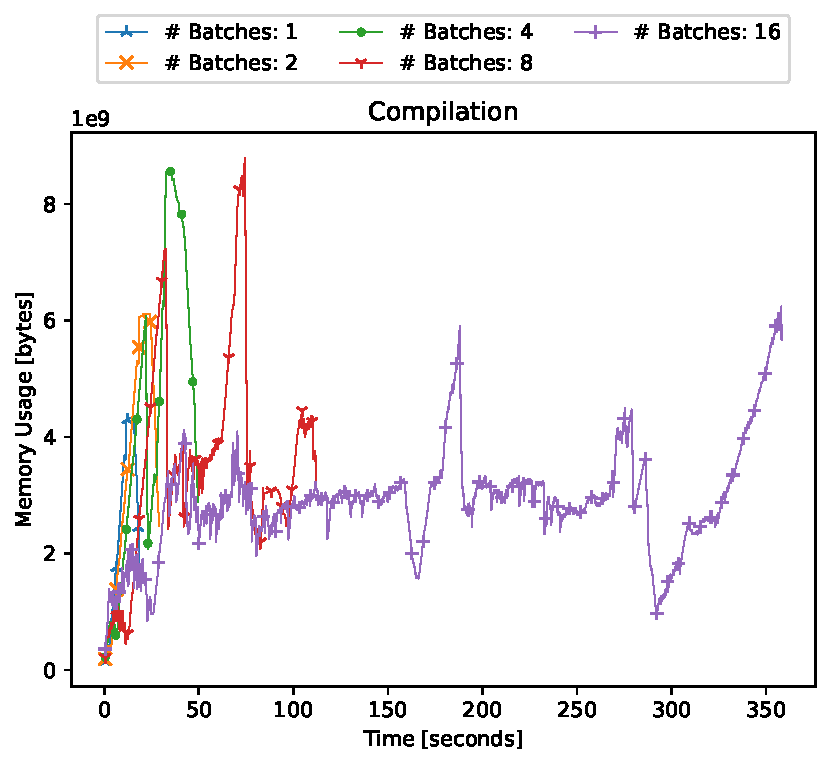
\includegraphics[width=1\textwidth]{benchmarks/compilation.pdf}
        \caption{$y=x$}
        \label{fig:y equals x}
    \end{subfigure}
    \hfill
    \begin{subfigure}[t]{0.49\textwidth}
        \centering
        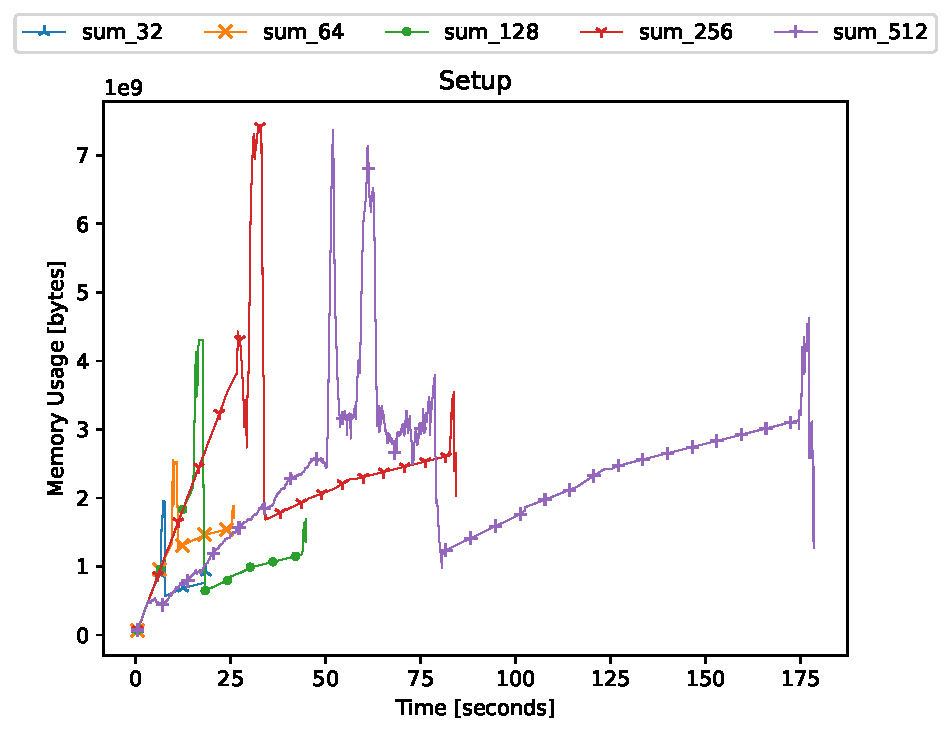
\includegraphics[width=1\textwidth]{benchmarks/setup.pdf}
        \caption{$y=x$}
        \label{fig:setup-graph}
    \end{subfigure}
    \caption{Three simple graphs}
    \label{fig:setup-phase}
\end{figure}

In addition to the off-chain computations, the setup phase includes the deployment of the on-chain verifier. Although the size of the verification key is relatively small, it takes up a significant amount of space in the resulting smart contract. The Ethereum mainnet introduced a smart contract size limit of 24.576 KB with EIP-170\footnote{https://eips.ethereum.org/EIPS/eip-170} in the Spurious Dragon hard-fork. While the verifier is converted to bytecode prior to deployment, thereby significantly reducing its size, the last two numbers of batches exceed the contract size limit due to large verification keys. This introduces an unexpected limit to the overall protocol as these verifiers cannot be deployed on the Ethereum blockchain. However, the verifier for the highest possible number of batches requires 3765288 Gas, which is rather expensive and approximately 12.5\% of the current 30 million block gas limit on the mainnet.

\begin{figure}[h]
    \centering
    \begin{subfigure}[t]{0.49\textwidth}
        \centering
        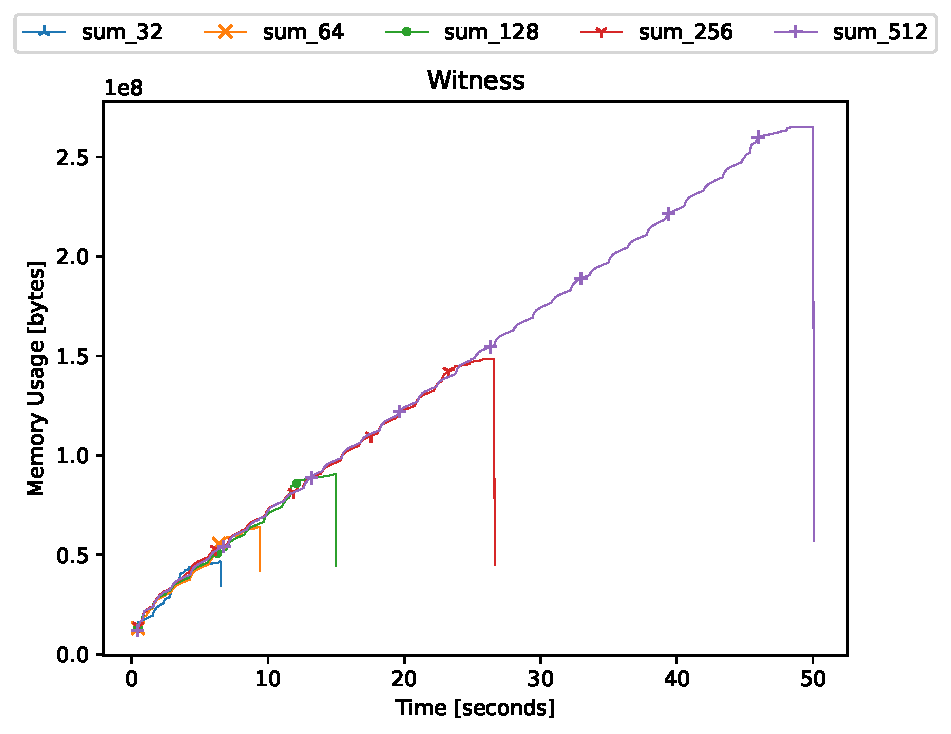
\includegraphics[width=1\textwidth]{benchmarks/witness.pdf}
        \caption{$y=x$}
        \label{fig:y equals x}
    \end{subfigure}
    \hfill
    \begin{subfigure}[t]{0.49\textwidth}
        \centering
        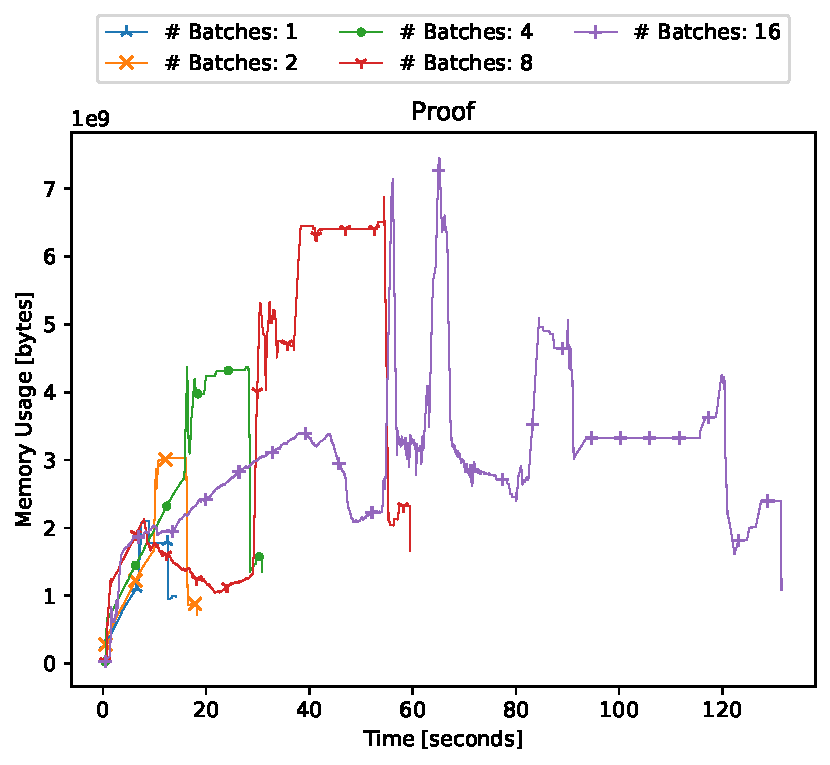
\includegraphics[width=1\textwidth]{benchmarks/proof.pdf}
        \caption{$y=x$}
        \label{fig:y equals x}
    \end{subfigure}
    \caption{Three simple graphs}
    \label{fig:three graphs}
\end{figure}

tabelle mit gas kosten

\section{Practical Feasibility}

- roundtrip time
- prices
- dataset size
- estimation of deployment costs for entire system? system anforderungen


\section{Threat Model}

- brute force, fairness, sybill attack?, 

vllt noch fairness? was muss buyer und was muss seller upfront zahlen?

geometrische folge 2^n

\section{Discussion}

- feasibility
- threat model

extra chapter?